\chapter{Results - Implementation}

\label{ch:implementationresults}

blablabla dass die das ergebnis von --langem-- rumprobieren sind

%############################################################################################
\section{Possible vectors}
%############################################################################################

\label{ch:thevectors}

%-progressvec (progress, laptime, lapcount, validvec)
%-speedsteer (motortorques, steerangle, velocity, fRightDirection, velocity of perpendiculars, angle, speedinstreetdir, speedintraversedir, cuvinessbeforecar)
%-carstatusvec (longitutinal and latidutialn slip for each tire)
%-centerdist, als vector
%-waldistvec (direction the car faces, steers, moves..... and directiont the street goes (each longsighted and shortsighted from car and streetmiddle)
%-lookahead-vector
%-delta und feedback
%-actual action (possibly overwritten)
%-both vision-vectors

\term{Possible Vectors} refers to all information the game streams over its socket to the agent. While most of this information will be used to make up an agent's state, the vectors also provide information about if the game must be reset as well as information to calculate the reward from. This information is collected in Unity in the function \codefunc{GetAllInfos()}, and converted into a namedtuple-wrapper called \codeobj{Otherinputs}, specified in \filename{read\_supervised.py}. In this section, I provide an overview of those vectors and their meaning in the game. I refer to the individual possible vectors by the name used in \codeobj{Otherinputs}.

\paragraph{ProgressVec} This vector contains information about the current progress of the car on the track, which consists of the actual progress in percent, the time the car needed for the current lap so far, the number of the current lap, as well as the flag if the round is still valid (which is the case if the car did not leave the street yet).

\paragraph{SpeedSteer} In this vector, information about the car's velocity and its steer angle is encoded. It consists of the following values:

\renewcommand{\arraystretch}{1.3}
\begin{flushleft}
	\begin{tabular}{>{\em}p{2.9cm} p{\textwidth-3.8cm}} 
		RLTorque & The motor torque applied to the left back tire\\
		RRTorque & The motor torque applied to the right back tire\\
		FLSteer & The steering angle of the front left tire\\
		FRSteer & The steering angle of the front right tire\\
		velocity & The velocity of the car as scalar independent of directions\\
		rightDirection & A boolean value if the car moves into the intended direction\\
		velocityOfPerpendiculars & \hspace*{0.8cm} The velocity of the orthogonal projection of the car onto the center of the street\\ %TODO see sectionbalabla, wo ich DOCH die definition von perpendicular einführen werde
		carAngle & The car's angle (in degrees) in relation to the street's direction\\
		speedInStreetDir & The car's velocity into the street's direction (calculated using the dot-product between the car's velocity-vectors and the direction-vector of the street at the car's current position)\\
		speedInTraverDir &  The car's velocity into the orthogonal of the street's direction\\
		CurvinessBeforeCar & A measure of the curvature of the street immediately ahead of the car ($CurvinessBeforeCar \in [0,1]$, where a value of zero corresponds to a straight street)\\	
	\end{tabular}
\end{flushleft}

\paragraph{StatusVector} This vector contains eight values, corresponding to the forward slip and sideways slip of each of the car's tires, using a function provided for Unity's \codeobj{WheelCollider}-object. The more the car slips, the smaller the impact of movement commands. The current slip-values are presented in the GUI of the game (and can be seen behind annotation \textbf{R} in figure~\ref{fig:aidriveshot}).

\paragraph{CenterDist and CenterDistVec} The \emph{CenterDist} corresponds to the car's orthogonal distance to the street's center, as calculated in \colorbox{red}{where} (also visually represented in the car's GUI, behind annotation \textbf{N} in figure~\ref{fig:aidriveshot}).
The \emph{CenterDistVec} contains the same information presented in another way: It is a vector of length 15, where the middle element corresponds to the car's longitutional position. The other elemnts correspond to points with regular distances to the car's left and right. The value of each respective element is calculated using the reversed distance between this position and the longitudional center of the street. The content of this vector is visually represented behind annotation \textbf{M} in figure~\ref{fig:aidriveshot}.

\paragraph{WallDistVec} This vector contains seven values, corresponding to the car's distance to the wall along a certain ray. It does not contain the closest distance to the wall -- because this value is already represented by the CenterDist. As the wall has always a fixed distance from the street's center (with an absolute value of five), the distance to the closest wall can be calculated as $5 - abs(CenterDist)$. 
For the calculation of the \emph{WallDistVec}, several rays are casted from the car's (or the perpendicular's) position into a particular direction. Returned is then the distance from their respective origin and their first intersection with a wall. The vector contains seven values, using rays with different origins and different directions. In the following table, I provide an explanation of each of those values, while figure~\ref{fig:walldistvec} in appendix~\ref{AppendixB} visually represents these rays. The respective color is mentioned in the table.
\renewcommand{\arraystretch}{1.3}
\begin{flushleft}
	\begin{tabular}{p{0.5cm} p{2cm} p{2.4cm} p{\textwidth-6.45cm}} 
		\# & color in \ref{fig:walldistvec} & origin & direction \\
		\hline
		1 & \textcolor{black}{black} & car's center & direction the car faces \\
		2 & \textcolor{magenta}{magenta} & car's center & direction the car steers\\	
		3 & \textcolor{red}{red} & car's center & direction the car moves\\	
		4 & \textcolor{black}{white} & car's center & short-sighted direction of the street (calculated as the vector between the closest \codeobj{anchorVector} behind the car and the closest one before the car) \\		
		5 & \textcolor{yellow}{yellow} & perpendicular & short-sighted direction of the street (calculated as the vector between the closest \codeobj{anchorVector} behind the car and the closest one before the car) \\
		6 & \textcolor{blue}{blue} & car's center & long-sighted direction of the street (calculated as the vector between the closest \codeobj{anchorVector}  to the car and the one 5 in advance) \\
		7 & \textcolor{gray}{gray} & perpendicular & long-sighted direction of the street (calculated as the vector between the closest \codeobj{anchorVector}  to the car and the one 5 in advance) \\
	\end{tabular}
\end{flushleft}

\paragraph{LookAheadVec} This vector corresponds to the course of the street ahead of the car. It is a vector consisting of 30 elements, corresponding to regularly spaced \codeobj{anchorVector}s, starting at the position of the car, following the direction of the street. The value at each position $i$ of this vector corresponds to the angle between the direction of the street at position $i$ and the direction at position $i+1$. In other words, if the street makes a shart turn 4 units ahead of the car, then element $3$ will contain a high value. The angle is measured in degrees. A graphical representation of this vector can be seen behind annotation \textbf{N} in figure~\ref{fig:aidriveshot}.

\paragraph{FBDelta} This vector consists of two values, namely \emph{Feedback} and \emph{Delta}. The Feedback-value is the temporal difference of how long the car needed for a specific section of the course (constrained via the closest \codeobj{anchorVector}s of the car) in the current process in comparison to the time needed in the fastest lap so far. The Delta-value is the absolute difference in time needed for the entire lap so far.

As both of these values are only useful in relation to the time needed for the fastest lap, it must be ensured that this does not change during training. For that, The file \filename{AiInterface.cs} contains in its class \codeobj{Consts} a flag \codeobj{lock\_fastestlap\_in\_AIMode}. Note however, that even if this flag is set, the values of \emph{FBDelta} could at most be used to calculate the agent's reward and not as part of its state.

\paragraph{Action} This is a three-dimensional vector corresponding to the actual action the environment recorded. While the agent knows what action it provided, it could be manually overwritten (after the press of \keystroke{H}) -- which is why the agent stores this vector in its replay memory instead of the action it would have performed otherwise.


\paragraph{Mini-maps} While the content of the mini-maps is not contained in the namedtuple \codeobj{Otherinput}, their value is transmitted from the game just like the other vectors. In the current implementation, both cameras have a resolution of $30\times45$ pixels, where one camera is $15$ units away of the car, and the other one $75$ units, which means that the former provides a smaller but more detailed view of the car. The closer camera is mostly referred to as $vvec2$, whereas the other one is denoted $visionvec$ or $vvec$.\\

As a working game was already provided by \leon of this thesis, so were some of these vectors, namely the calculation of FBDelta, LookAheadVec, CenterDist and CenterDistVec, as well as many elements necessary to compute many of the other ones. 
It is worth noting that most \term{possible vectors} are normalized after loading, according to (in part estimated) minimal- and maximal values, such that all their values in [0,1]. The corresponding \codeobj{MINVALS} and \codeobj{MAXVALS} are defined in \filename{read\_supervised.py}

%############################################################################################
\section{Implemented Models}
%############################################################################################

One has to be aware that the DQN-models need the agent to be discretized to a one-hot vector, while the DDPQ-models need the action input in form of three real numbers. As in the current implementation both models are used by respective agents, this function may have to be overwritten

No pooling, nur stride

There are two different models implemented in this project: a \keyword{Double Dueling Deep-Q-Learning} model, specified in the class \codeobj{DDDQN\_model} in \filename{models/dddqn.py}\footnote{\url{https://github.com/cstenkamp/BA-rAIce-ANN/blob/master/models/dddqn.py}} as well as a \keyword{Deep Deterministic Policy Gradient} model, specified in \codeobj{DDPG\_model} in \filename{models/ddpg.py}\footnote{\url{https://github.com/cstenkamp/BA-rAIce-ANN/blob/master/models/ddpg.py}} Both models learn via temporal differences and are in detail explained in chapters~\ref{ch:DQN}ff and \ref{ch:ddpg}, respectively. 

While the actual learning technique differs in both models, they both implement the same interface (not implemented because of python's duck typing), such that the functions relevant for the agent are accessible in the same way. An UML-diagram of most of their functions as well as the interface is given in figure~\ref{fig:modelssmall}. 

\begin{figure}[h]
	\centering 
	\includegraphics[width=\textwidth]{uml_diagrams/models_inText2.2}
	\caption{UML-diagram of the two given models as well as the interface both of them implement}
	\label{fig:modelssmall}
\end{figure}

Both implemented models provide the possibility to load and save a model from/to the harddisk unsing TensorFlow's saver-class. If a model is loaded in the \codeother{isPretrain}-mode, it can be saved to file and loaded again such that it is usable. If the model is saved, the information about its already performed numbers of inferences and learning-steps are saved within TensorFlow as well. When a model is saved, it saves into the directory \codeobj{conf.pretrain\_checkpoint\_dir} if the respective flag is set, and \codeobj{conf.checkpoint\_dir} else. When loading a model (in \codefunc{initNet(load)}), the \codefunc{load}-parameter specifies if the model should be loaded from the pretrain-directory, the non-pretrain-directory, the newest one of those or none at all.




blablabla überleitung dass ich jetzt erst das eine dann das andere erläutere

\paragraph{DQN-model}

DASS DISKRETISIERT WIRD; WTF WIE KONNTE ICH DAS NOCH NICHT ERWÄHNT HABEN

The class \codeobj{DDDQN\_model} \term{has} two \codeobj{DuelDQN}s, which are Deep Convolutional Neural Networks with Dueling Architectures, specified as computational graph using TensorFlow -- one of them being its online network, and the other the target network. The \codeobj{DDDQN\_model} combines then for the learning method of Double-Q-Learning (as detailed in section~\ref{ch:DQN}ff as well as appendix~\ref{AppendixA}) in its method \codefunc{q\_train\_step}. 

The provided DQN-model can however not only learn via Q-learning, but can also be trained supervisedly. For that, it also specifies the function \codefunc{sv\_train\_step}. This method can only be called if \codeobj{isPretrain} and learns directly on its target network. For that, the used \codeobj{DuelDQN}s must provide a TensorFlow-placeholder for the target-action.

blablabla die settozero-function

Its network-architecture is specified in the next section.





-auf die gym\_test klasse eingehen mit der man testen kann ob man das model abgefuckt hat
-das uml-diagramm
-das krasse schlecte diskretisieren in dqn-based, inkl course of dimensionality und allem!\\


\subsubsection{Network architecture}

\paragraph{DQN}

An overview of the general network architecture, as used by the \codeobj{dqn\_rl\_agent}, is provided in figure~\ref{fig:dqn_graph}. Note however that the actual architecture differs in other agents, as it depends on the agent's configuration of \term{features}. Some agents do not use the minimaps as input, their implementation therefore does not use any of the convolutional layers from the upper line of the figure.

\begin{figure}[h]
	\centering 
	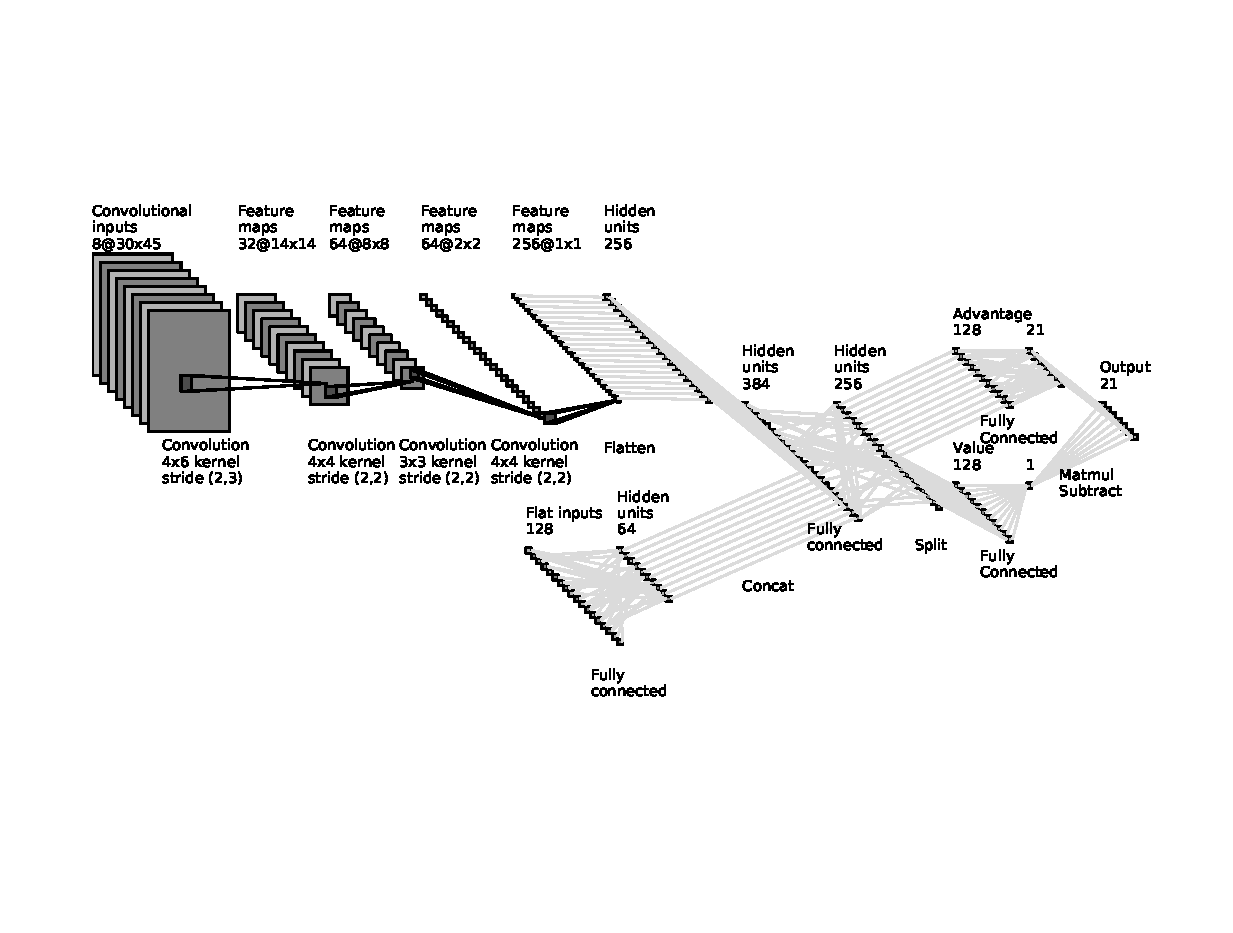
\includegraphics[trim={1.22cm 3.4cm 1.15cm 3cm},clip,width=1.05\textwidth]{draw_convnet/dqn}
	\caption{The used convolutional DQN-network with a dueling architecture}
	\label{fig:dqn_graph}
\end{figure}


\begin{figure}[h]
	\centering 
	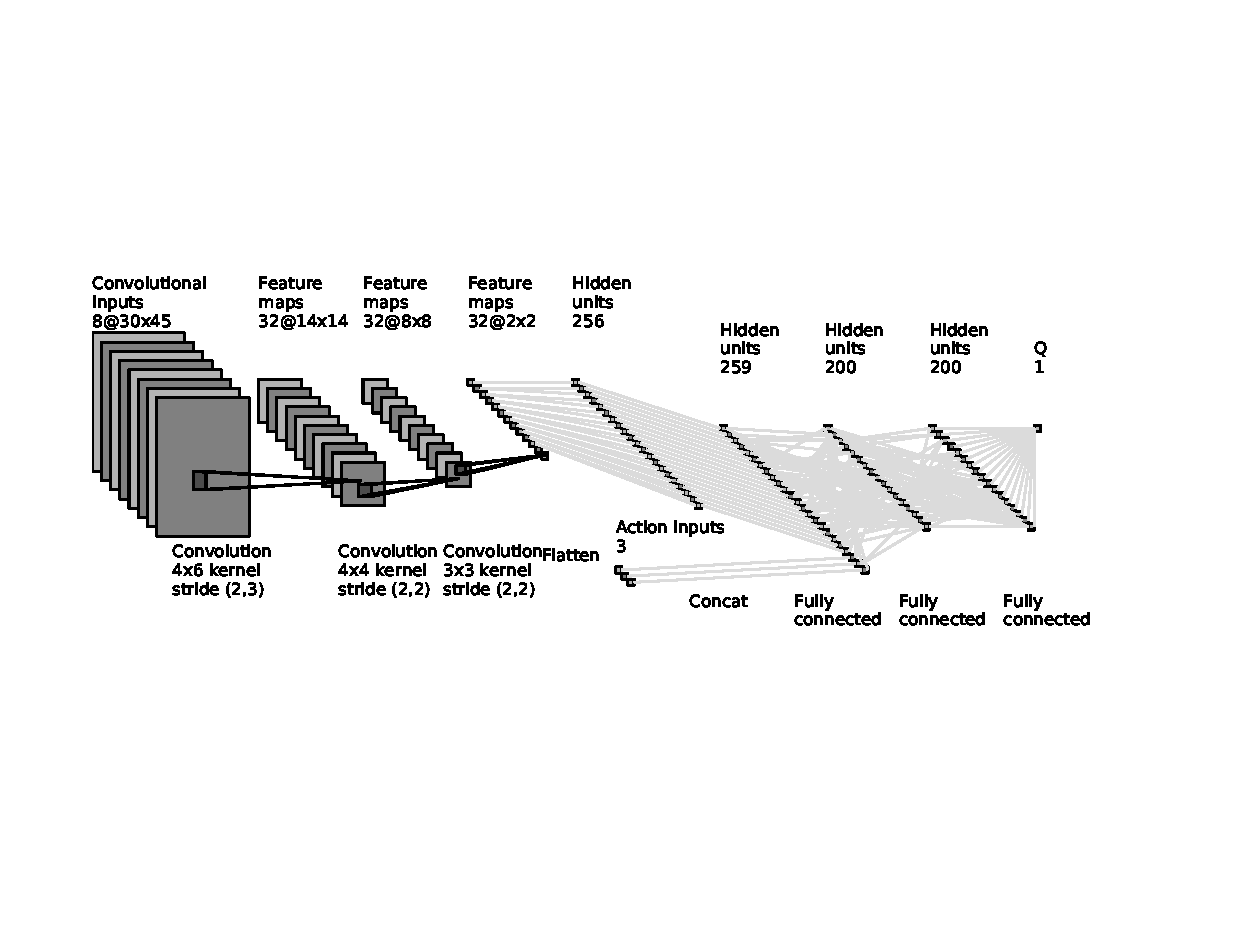
\includegraphics[trim={1.22cm 4.6cm 2cm 3cm},clip,width=1.05\textwidth]{draw_convnet/critic-2d}
	\caption{Convolutional critic}
	\label{fig:2dcrit}
\end{figure}

\begin{figure}[h]
	\centering 
	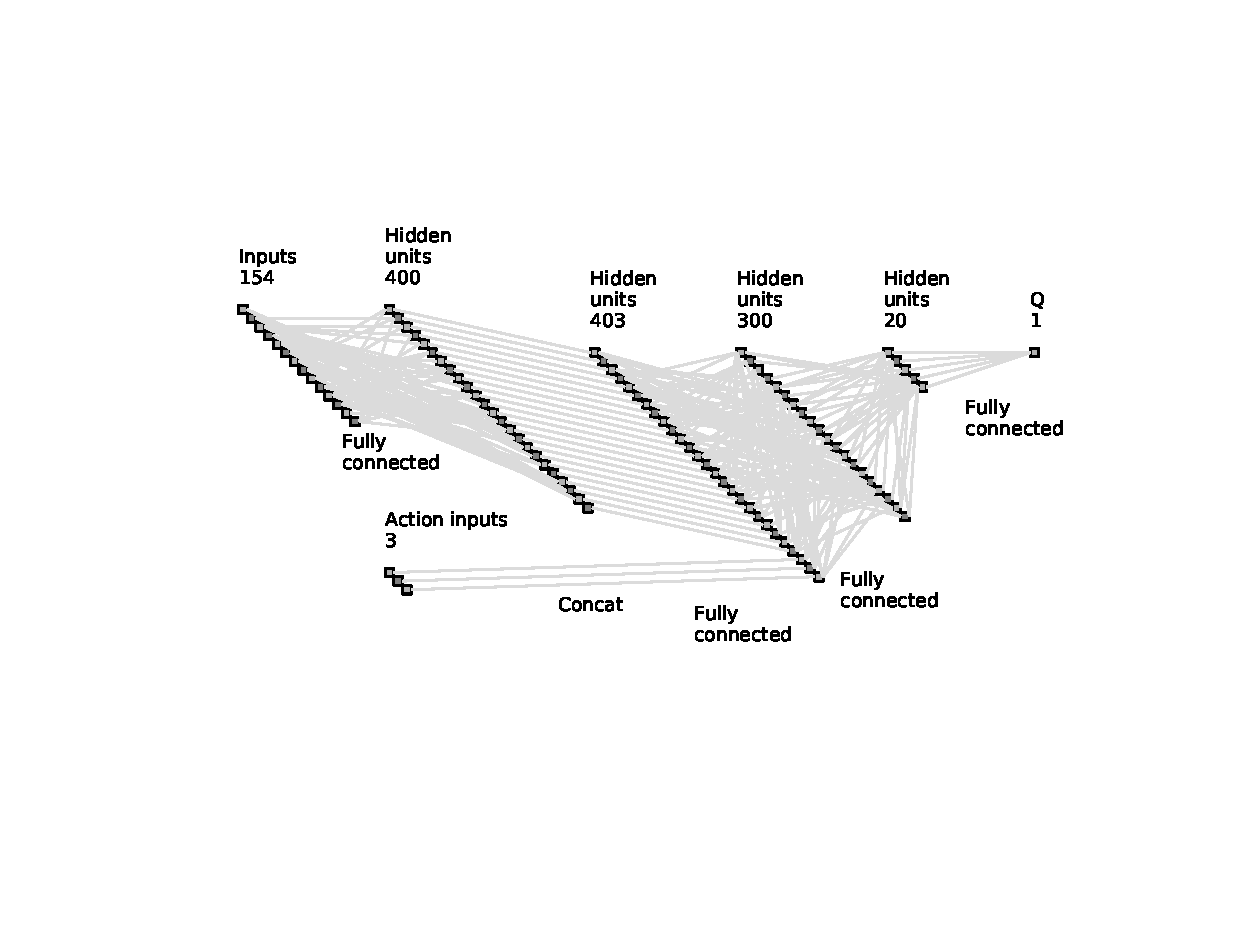
\includegraphics[trim={3.7cm 4.4cm 2cm 3cm},clip,width=1.05\textwidth]{draw_convnet/critic-lowd}
	\caption{Low-dimensional critic}
	\label{fig:lowcrit}
\end{figure}

\begin{figure}[h]
	\centering 
	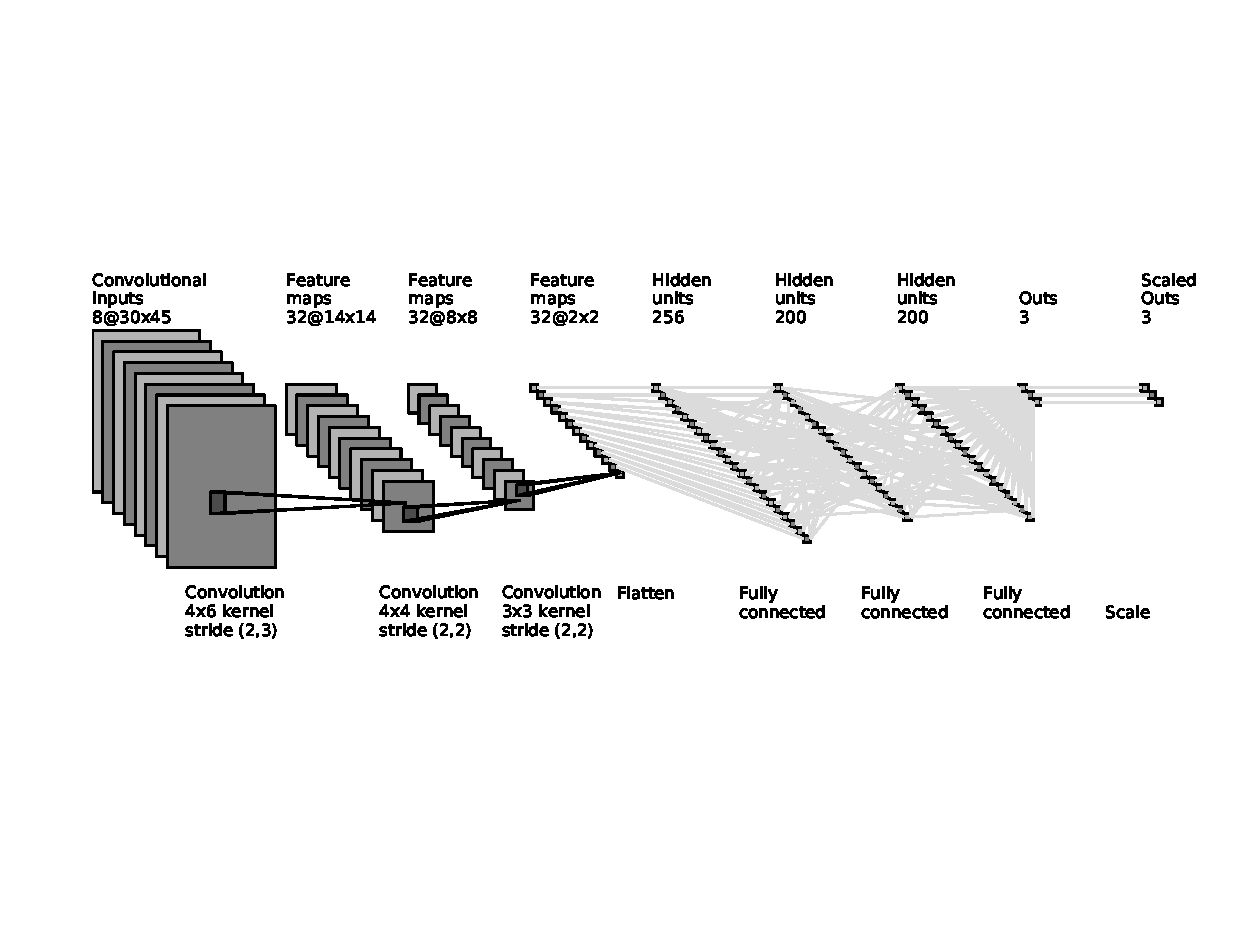
\includegraphics[trim={1.22cm 5.03cm 0.4cm 3cm},clip,width=1.05\textwidth]{draw_convnet/actor-2d}
	\caption{Convolutional actor}
	\label{fig:2dact}
\end{figure}

\begin{figure}[h]
	\centering 
	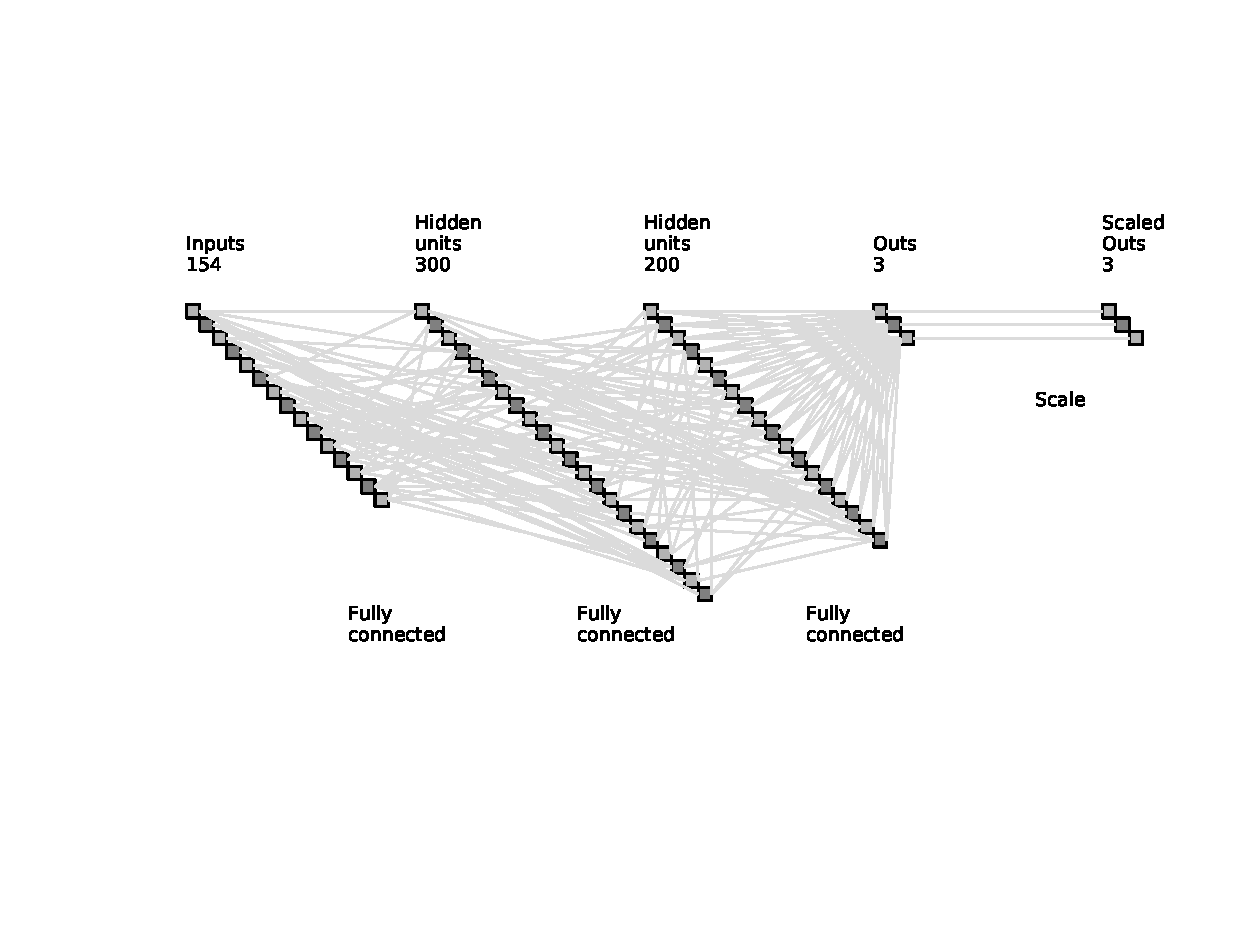
\includegraphics[trim={2.7cm 4.2cm 0.8cm 3cm},clip,width=1.05\textwidth]{draw_convnet/actor-lowd}
	\caption{Low-dimensional actor}
	\label{fig:lowdact}
\end{figure}

In a hybrid ANN (having both 2D and 1D input), four convolutional layers calculate an abstract representation of the two-dimensional inputs, which is flattened into a hidden layer consisting of 256 Units. The one-dimensional input are connected via a dense layer to another hidden layer of 64 units. These two layers are then concatenated to form a layer of 384 hidden Units, which is densely connected to a furhter hidden layer, which splits into an advantage and a value stream as proposed by \cite{wang_dueling_2015}. While the advantage stream ends in a layer with one unit for each action, the value-stream has one output. In the very last layer of the network, the advantage and value stream are combined into the final output layer, providing a separate Q-value for each action.



1. dqn-algorithm
- anzahl layer, Batchnorm, doubles dueling
- clipping wieder rein, reference auf das dueling
- grundsätzlich gegen batchnorm entschieden, siehe reddit post
- MIT GRAFIK
- Adam und tensorflow quoten, siehe zotero
2. ddpg
- anzahl layer, Batchnorm
- MIT GRAFIK

-mo
-schöne grafik.
-auf meien DQN-config eingehen und(!!!) ne DDPG-config machen, using the "experiment details" vom ddpg paper  


In the original DDPG-algorithm \cite{lillicrap_continuous_2015}, the authors used \keyword{batch normalization} \cite{ioffe_batch_2015} to have the possibility of using the same network hyperparameters for differently scaled input-values. In the learning step when using minibatches, \batchnorm normalizes each dimension across the samples in a batch to have unit mean and variance, whilst keeping a running mean and variance to normalize in non-learning steps. In Tensorflow, batchnorm can be added with an additional layer and an additional input, specifying the phase (learning step/non-learning step)\footnote{cf. \url{https://www.tensorflow.org/api\_docs/python/tf/contrib/layers/batch_norm}}. Though Lillicrap et al. seemed to have success on using \batchnorm, in practice it lead to unstability, even on simple physics tasks in openAI's gym. As I am not the only one having this issue \footnote{redditlink}, I left out batch normalization for good.





\paragraph{DDPG}

-die grafik von andrea
-satz über batchnorm

%############################################################################################
\section{Implemented Agents}
d%############################################################################################

\begin{tabular}{l l l l}
	filename & uses model & uses visionvector & performs RL\\
	\hline
	\textbf{ddpg\_novision\_rl\_agent}.py & DDPG & no & yes\\	
	\textbf{ddpg\_rl\_agent}.py & DDPG & yes & yes\\
	\textbf{dqn\_novision\_rl\_agent}.py & DQN & no & yes\\
	\textbf{dqn\_rl\_agent}.py & DQN & yes & yes\\
	\textbf{dqn\_sv\_agent}.py & \blap{supervised network\\ with DQN-structure} & yes & no\\[2em]
\end{tabular}


\subsection{Pretraining}

\subsection{Exploration}

Only very basic exploration algorithms are provided in this thesis. There are two different methods used in the DQN-based agents compared to the agents with a DDPG-model, following their definition of an action. While in DDPG-based agents it holds that $action \subset \mathds{R}^{n \in \mathds{N}}$, in DQN-based agent the action is discretized into one unique value. 

While the action-value 

-epsilon-greedy als standard und make_noisy vom DDPG


\subsection{Reward}

-meine theorien: continuous, non-negative, aus ner shclehcten darf nicht besser sein als in einem guten eh sein)
-dass immer speed belohnen negativ ist, siehe ->problem bei ddpg, approach von dem kerastorcsguy, siehe kapitel \colorbox{red}{Daskapitel}
-die funktion wo man sich den durchgängingen reward in ner farbe plotten kann (auch bei \keystroke{H})

\subsection{Observation}




\subsection{Performance measure}

% TODO -dass halt eigentlich zu jedem zeitpunkt compared zu rrt oder human sein müsste